\documentclass[a4paper,14pt,oneside,openany]{memoir}

%%% Задаем поля, отступы и межстрочный интервал %%%

\usepackage[left=30mm, right=15mm, top=20mm, bottom=20mm]{geometry} % Пакет geometry с аргументами для определения полей
\pagestyle{plain} % Убираем стандарные для данного класса верхние колонтитулы с заголовком текущей главы, оставляем только номер страницы снизу по центру
\parindent=1.25cm % Абзацный отступ 1.25 см, приблизительно равно пяти знакам, как по ГОСТ
\usepackage{indentfirst} % Добавляем отступ к первому абзацу
%\linespread{1.3} % Межстрочный интервал (наиболее близко к вордовскому полуторному) - тут вместо этого используется команда OnehalfSpacing*

%%% Задаем языковые параметры и шрифт %%%

\usepackage[english, russian]{babel}                % Настройки для русского языка как основного в тексте
\babelfont{rm}{Times New Roman}                     % TMR в качестве базового roman-щрифта

%%% Задаем стиль заголовков и подзаголовков в тексте %%%

\setsecnumdepth{subsection} % Номера разделов считать до третьего уровня включительно, т.е. нумеруются только главы, секции, подсекции
\renewcommand*{\chapterheadstart}{} % Переопределяем команду, задающую отступ над заголовком, чтобы отступа не было
\renewcommand*{\printchaptername}{} % Переопределяем команду, печатающую слово "Глава", чтобы оно не печалось
%\renewcommand*{\printchapternum}{} % То же самое для номера главы - тут не надо, номер главы оставляем
\renewcommand*{\chapnumfont}{\normalfont\bfseries} % Меняем стиль шрифта для номера главы: нормальный размер, полужирный
\renewcommand*{\afterchapternum}{\hspace{1em}} % Меняем разделитель между номером главы и названием
\renewcommand*{\printchaptertitle}{\normalfont\bfseries\centering\MakeUppercase} % Меняем стиль написания для заголовка главы: нормальный размер, полужирный, центрированный, заглавными буквами
\setbeforesecskip{20pt} % Задаем отступ перед заголовком секции
\setaftersecskip{20pt} % Ставим такой же отступ после заголовка секции
\setsecheadstyle{\raggedright\normalfont\bfseries} % Меняем стиль написания для заголовка секции: выравнивание по правому краю без переносов, нормальный размер, полужирный
\setbeforesubsecskip{20pt} % Задаем отступ перед заголовком подсекции
\setaftersubsecskip{20pt} % Ставим такой же отступ после заголовка подсекции
\setsubsecheadstyle{\raggedright\normalfont\bfseries}  % Меняем стиль написания для заголовка подсекции: выравнивание по правому краю без переносов, нормальный размер, полужирный

%%% Задаем параметры оглавления %%%

\addto\captionsrussian{\renewcommand\contentsname{Содержание}} % Меняем слово "Оглавление" на "Содержание"
\setrmarg{2.55em plus1fil} % Запрещаем переносы слов в оглавлении
%\setlength{\cftbeforechapterskip}{0pt} % Эта команда убирает интервал между заголовками глав - тут не надо, так красивее смотрится
\renewcommand{\aftertoctitle}{\afterchaptertitle \vspace{-\cftbeforechapterskip}} % Делаем отступ между словом "Содержание" и первой строкой таким же, как у заголовков глав
%\renewcommand*{\chapternumberline}[1]{} % Делаем так, чтобы номер главы не печатался - тут не надо
\renewcommand*{\cftchapternumwidth}{1.5em} % Ставим подходящий по размеру разделитель между номером главы и самим заголовком
\renewcommand*{\cftchapterfont}{\normalfont\MakeUppercase} % Названия глав обычным шрифтом заглавными буквами
\renewcommand*{\cftchapterpagefont}{\normalfont} % Номера страниц обычным шрифтом
\renewcommand*{\cftchapterdotsep}{\cftdotsep} % Делаем точки до номера страницы после названий глав
\renewcommand*{\cftdotsep}{1} % Задаем расстояние между точками
\renewcommand*{\cftchapterleader}{\cftdotfill{\cftchapterdotsep}} % Делаем точки стандартной формы (по умолчанию они "жирные")
\maxtocdepth{subsection} % В оглавление попадают только разделы первыхтрех уровней: главы, секции и подсекции

%%% Выравнивание и переносы %%%

%% http://tex.stackexchange.com/questions/241343/what-is-the-meaning-of-fussy-sloppy-emergencystretch-tolerance-hbadness
%% http://www.latex-community.org/forum/viewtopic.php?p=70342#p70342
\tolerance 1414
\hbadness 1414
\emergencystretch 1.5em                             % В случае проблем регулировать в первую очередь
\hfuzz 0.3pt
\vfuzz \hfuzz
%\dbottom
%\sloppy                                            % Избавляемся от переполнений
\clubpenalty=10000                                  % Запрещаем разрыв страницы после первой строки абзаца
\widowpenalty=10000                                 % Запрещаем разрыв страницы после последней строки абзаца
\brokenpenalty=4991                                 % Ограничение на разрыв страницы, если строка заканчивается переносом

%%% Объясняем компилятору, какие буквы русского алфавита можно использовать в перечислениях (подрисунках и нумерованных списках) %%%
%%% По ГОСТ нельзя использовать буквы ё, з, й, о, ч, ь, ы, ъ %%%
%%% Здесь также переопределены заглавные буквы, хотя в принципе они в документе не используются %%%

\makeatletter
    \def\russian@Alph#1{\ifcase#1\or
       А\or Б\or В\or Г\or Д\or Е\or Ж\or
       И\or К\or Л\or М\or Н\or
       П\or Р\or С\or Т\or У\or Ф\or Х\or
       Ц\or Ш\or Щ\or Э\or Ю\or Я\else\xpg@ill@value{#1}{russian@Alph}\fi}
    \def\russian@alph#1{\ifcase#1\or
       а\or б\or в\or г\or д\or е\or ж\or
       и\or к\or л\or м\or н\or
       п\or р\or с\or т\or у\or ф\or х\or
       ц\or ш\or щ\or э\or ю\or я\else\xpg@ill@value{#1}{russian@alph}\fi}
\makeatother

%%% Задаем параметры оформления рисунков и таблиц %%%

\usepackage{graphicx, caption, subcaption} % Подгружаем пакеты для работы с графикой и настройки подписей
\graphicspath{{images/}} % Определяем папку с рисунками
\captionsetup[figure]{font=small, width=\textwidth, name=Рисунок, justification=centering} % Задаем параметры подписей к рисункам: маленький шрифт (в данном случае 12pt), ширина равна ширине текста, полнотекстовая надпись "Рисунок", выравнивание по центру
\captionsetup[subfigure]{font=small} % Индексы подрисунков а), б) и так далее тоже шрифтом 12pt (по умолчанию делает еще меньше)
\captionsetup[table]{singlelinecheck=false,font=small,width=\textwidth,justification=justified} % Задаем параметры подписей к таблицам: запрещаем переносы, маленький шрифт (в данном случае 12pt), ширина равна ширине текста, выравнивание по ширине
\captiondelim{ --- } % Разделителем между номером рисунка/таблицы и текстом в подписи является длинное тире
\setkeys{Gin}{width=\textwidth} % По умолчанию размер всех добавляемых рисунков будет подгоняться под ширину текста
\renewcommand{\thesubfigure}{\asbuk{subfigure}} % Нумерация подрисунков строчными буквами кириллицы
%\setlength{\abovecaptionskip}{0pt} % Отбивка над подписью - тут не меняем
%\setlength{\belowcaptionskip}{0pt} % Отбивка под подписью - тут не меняем
\usepackage[section]{placeins} % Объекты типа float (рисунки/таблицы) не вылезают за границы секциии, в которой они объявлены

%%% Задаем параметры ссылок и гиперссылок %%% 

\usepackage{hyperref}                               % Подгружаем нужный пакет
\hypersetup{
    colorlinks=true,                                % Все ссылки и гиперссылки цветные
    linktoc=all,                                    % В оглавлении ссылки подключатся для всех отображаемых уровней
    linktocpage=true,                               % Ссылка - только номер страницы, а не весь заголовок (так выглядит аккуратнее)
    linkcolor=red,                                  % Цвет ссылок и гиперссылок - красный
    citecolor=red                                   % Цвет цитировний - красный
}

%%% Настраиваем отображение списков %%%

\usepackage{enumitem}                               % Подгружаем пакет для гибкой настройки списков
\renewcommand*{\labelitemi}{\normalfont{--}}        % В ненумерованных списках для пунктов используем короткое тире
\makeatletter
    \AddEnumerateCounter{\asbuk}{\russian@alph}     % Объясняем пакету enumitem, как использовать asbuk
\makeatother
\renewcommand{\labelenumii}{\asbuk{enumii})}        % Кириллица для второго уровня нумерации
\renewcommand{\labelenumiii}{\arabic{enumiii})}     % Арабские цифры для третьего уровня нумерации
\setlist{noitemsep, leftmargin=*}                   % Убираем интервалы между пунками одного уровня в списке
\setlist[1]{labelindent=\parindent}                 % Отступ у пунктов списка равен абзацному отступу
\setlist[2]{leftmargin=\parindent}                  % Плюс еще один такой же отступ для следующего уровня
\setlist[3]{leftmargin=\parindent}                  % И еще один для третьего уровня

%%% Счетчики для нумерации объектов %%%

\counterwithout{figure}{chapter}                    % Сквозная нумерация рисунков по документу
\counterwithout{equation}{chapter}                  % Сквозная нумерация математических выражений по документу
\counterwithout{table}{chapter}                     % Сквозная нумерация таблиц по документу

%%% Реализация библиографии пакетами biblatex и biblatex-gost с использованием движка biber %%%

\usepackage{csquotes} % Пакет для оформления сложных блоков цитирования (biblatex рекомендует его подключать)
\usepackage[%
backend=biber,                                      % Движок
bibencoding=utf8,                                   % Кодировка bib-файла
sorting=none,                                       % Настройка сортировки списка литературы
style=gost-numeric,                                 % Стиль цитирования и библиографии по ГОСТ
language=auto,                                      % Язык для каждой библиографической записи задается отдельно
autolang=other,                                     % Поддержка многоязычной библиографии
sortcites=true,                                     % Если в квадратных скобках несколько ссылок, то отображаться будут отсортированно
movenames=false,                                    % Не перемещать имена, они всегда в начале библиографической записи
maxnames=5,                                         % Максимальное отображаемое число авторов
minnames=3,                                         % До скольки сокращать число авторов, если их больше максимума
doi=false,                                          % Не отображать ссылки на DOI
isbn=false,                                         % Не показывать ISBN, ISSN, ISRN
]{biblatex}[2016/09/17]
\DeclareDelimFormat{bibinitdelim}{}                 % Убираем пробел между инициалами (Иванов И.И. вместо Иванов И. И.)
\addbibresource{biba.bib}                           % Определяем файл с библиографией

%%% Скрипт, который автоматически подбирает язык (и, следовательно, формат) для каждой библиографической записи %%%
%%% Если в названии работы есть кириллица - меняем значение поля langid на russian %%%
%%% Все оставшиеся пустые места в поле langid заменяем на english %%%

\DeclareSourcemap{
  \maps[datatype=bibtex]{
    \map{
        \step[fieldsource=title, match=\regexp{^\P{Cyrillic}*\p{Cyrillic}.*}, final]
        \step[fieldset=langid, fieldvalue={russian}]
    }
    \map{
        \step[fieldset=langid, fieldvalue={english}]
    }
  }
}

%%% Прочие пакеты для расширения функционала %%%

\usepackage{longtable,ltcaption}                    % Длинные таблицы
\usepackage{multirow,makecell}                      % Улучшенное форматирование таблиц
\usepackage{booktabs}                               % Еще один пакет для красивых таблиц
\usepackage{soulutf8}                               % Поддержка переносоустойчивых подчёркиваний и зачёркиваний
\usepackage{icomma}                                 % Запятая в десятичных дробях
\usepackage{hyphenat}                               % Для красивых переносов
\usepackage{textcomp}                               % Поддержка "сложных" печатных символов типа значков иены, копирайта и т.д.
\usepackage[version=4]{mhchem}                      % Красивые химические уравнения
\usepackage{amsmath}                                % Усовершенствование отображения математических выражений 
\usepackage{listings}
\usepackage{xcolor}
\usepackage{graphicx}
\usepackage{epstopdf} %%package to overcome problem with eps in pdf files
\usepackage{amsmath}
\usepackage{amsfonts}

\usepackage{mathtools}
\usepackage{xparse}

% \usepackage{amsthm}
% \usepackage{tcolorbox}
% \usepackage{floatrow}
% \usepackage{tabularx}
% % \usepackage[bottom]{footmisc} 
% \usepackage{titleps}
% \usepackage{breqn}
%%% Вставляем по очереди все содержательные части документа %%%

\begin{document}

\thispagestyle{empty}

\begin{center}
    МИНИСТЕРСТВО НАУКИ И ВЫСШЕГО ОБРАЗОВАНИЯ \\ РОССИЙСКОЙ ФЕДЕРАЦИИ

    \vspace{20pt}

    Университет ИТМО

    \vspace{20pt}

    Факультет систем управления и робототехники
\end{center}

\vfill

\begin{center}
    ОТЧЁТ \\  
    по дисциплине \\
    \textit{"Линейные системы автоматического управления"}

    \vspace{20pt}

    по теме: \\
    \uppercase{Формы представления линейных динамических систем}
\end{center}

\vfill

\noindent Студент: \\
\textit{Группа R3336 \hfill Поляков А.А.}


    \vspace{20pt}

    \noindent Предподаватель: \\
    \textit{к.т.н., доцент \hfill Перегудин А.А.}

\vfill

\begin{center}
    Санкт-Петербург \\ 2024
\end{center}                                     % Титульник

\newpage % Переходим на новую страницу
\setcounter{page}{2} % Начинаем считать номера страниц со второй
\OnehalfSpacing* % Задаем полуторный интервал текста (в титульнике одинарный, поэтому команда стоит после него)

\tableofcontents*                                   % Автособираемое оглавление

\chapter{Исходный код}
\label{ch:chap0}

\definecolor{codegreen}{rgb}{0,0.6,0}
\definecolor{codegray}{rgb}{0.5,0.5,0.5}
\definecolor{codepurple}{rgb}{0.58,0,0.82}
\definecolor{backcolour}{rgb}{0.95,0.95,0.92}

\lstdefinestyle{mystyle}{
    backgroundcolor=\color{backcolour},   
    commentstyle=\color{codegreen},
    keywordstyle=\color{magenta},
    numberstyle=\tiny\color{codegray},
    stringstyle=\color{codepurple},
    basicstyle=\ttfamily\footnotesize,
    breakatwhitespace=false,         
    breaklines=true,                 
    captionpos=b,                    
    keepspaces=true,                 
    numbers=left,                    
    numbersep=5pt,                  
    showspaces=false,                
    showstringspaces=false,
    showtabs=false,                  
    tabsize=2
}

\lstset{style=mystyle}

Запускал все симуляции симулинка через Live-script матлабовские, там же можно взглянуть на графики, в \href{https://github.com/GreedlyCore/control_theory_course}{репозитории} можно найти исходники. 

\endinput
\chapter{Одноканальная система в форме вход-выход}
\label{ch:chap1}

\definecolor{codegreen}{rgb}{0,0.6,0}
\definecolor{codegray}{rgb}{0.5,0.5,0.5}
\definecolor{codepurple}{rgb}{0.58,0,0.82}
\definecolor{backcolour}{rgb}{0.95,0.95,0.92}

\lstdefinestyle{mystyle}{
    backgroundcolor=\color{backcolour},   
    commentstyle=\color{codegreen},
    keywordstyle=\color{magenta},
    numberstyle=\tiny\color{codegray},
    stringstyle=\color{codepurple},
    basicstyle=\ttfamily\footnotesize,
    breakatwhitespace=false,         
    breaklines=true,                 
    captionpos=b,                    
    keepspaces=true,                 
    numbers=left,                    
    numbersep=5pt,                  
    showspaces=false,                
    showstringspaces=false,
    showtabs=false,                  
    tabsize=2
}

\lstset{style=mystyle}


В случае моего второго варианта получим следующее ДУ:
$$
\begin{aligned}
    \dddot{y} + 6\ddot{y} + 11\dot{y} + 6y = 6\ddot{u} + 4\dot{u} + 16u
\end{aligned}
$$

Для того, чтобы составить структурную схему, выполним несколько преобразований с ДУ - заменим дифференцирования на применение соответсвующих операторов, а после преобразуем в более удобный вид:

$$
\begin{aligned}
    p^3[y] + 6p^2[y] + 11p[y] + 6y = 6p^2[u] + 4p[u] + 16u \\
	y = \frac{1}{p^3} \bigg[ -6p^2[y] - 11p[y] -6y + 6p^2[u] + 4p[u] + 16u \bigg] \\
	y = -6\frac{1}{p}[y] - 11\frac{1}{p^2}[y] -6\frac{1}{p^3}[y] + 6\frac{1}{p}[u] + 4\frac{1}{p^2}[u] + 16\frac{1}{p^3}[u] \\
	y = \frac{1}{p}[-6y + 6u] + \frac{1}{p^2}[-11y + 4u] \frac{1}{p^3}[-6y + 16u]
\end{aligned}
$$
Так как блок "дифференцирования" в матлабе - довольно опасная штука, то воспользуемся классическим приёмом составления схем: от обратного, постепенно снижая степень дифференцирования у "игрека" посредством интегрирования. Снизу мы построили передаточную функцию от ДУ, чтобы проверить результат симуляции:

\newpage
В итоге, структурная схема системы, построенная в \textit{Simulink}:

\begin{figure}[ht]
    \centering
    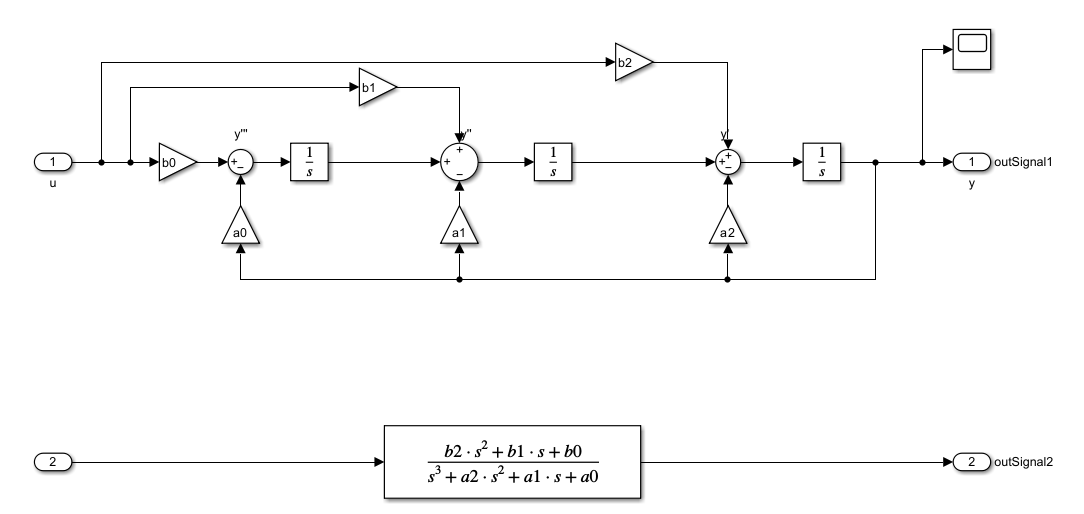
\includegraphics[width=1\textwidth]{scheme_task1.png}
	\caption{Схема системы}
\end{figure}

Подадим на такую схему сигнал $u(t)=1$ при нулевых начальных условиях: $\ddot{y}(0)=\dot{y}(0)=y(0)=0$. Графики сигналов, полученные на основе схемы:
\begin{figure}[ht]
    \centering
    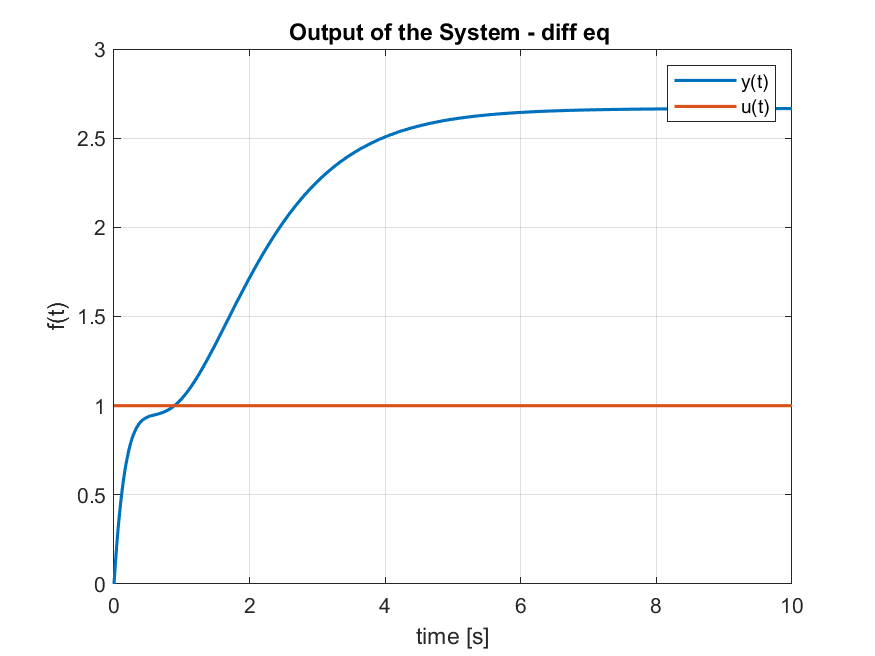
\includegraphics[width=0.5\textwidth]{output_task1_diff_eq.png}
	\caption{Симуляция - дифференциальное уравнение}
\end{figure}

Проверим полученный результат с помощью передаточной функции, её схема была выше, результат:
\begin{figure}[ht]
    \centering
    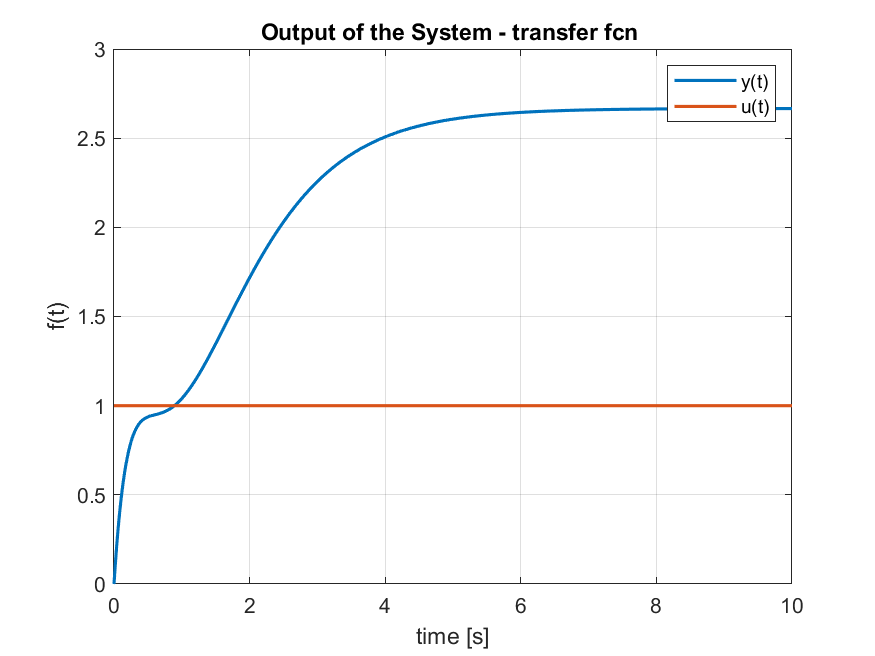
\includegraphics[width=0.5\textwidth]{output_task1_transfer_fcn.png}
	\caption{Симуляция - передаточная функция}
\end{figure}


\endinput
\chapter{Переход от формы вход-выход к форме вход-состояние-выход}
\label{ch:chap2}

\ExplSyntaxOn
\clist_new:N \l_feq_vector_clist
\NewDocumentCommand{\feqvector}{O{\\}mO{b}}{
  \clist_set:Nn \l_feq_vector_clist {#2} % Set the list
  \begin{#3matrix}
  \clist_use:Nn \l_feq_vector_clist {#1} % show it with separator from #1 (\\)
  \end{#3matrix}
}
\ExplSyntaxOff


\definecolor{codegreen}{rgb}{0,0.6,0}
\definecolor{codegray}{rgb}{0.5,0.5,0.5}
\definecolor{codepurple}{rgb}{0.58,0,0.82}
\definecolor{backcolour}{rgb}{0.95,0.95,0.92}

\lstdefinestyle{mystyle}{
    backgroundcolor=\color{backcolour},   
    commentstyle=\color{codegreen},
    keywordstyle=\color{magenta},
    numberstyle=\tiny\color{codegray},
    stringstyle=\color{codepurple},
    basicstyle=\ttfamily\footnotesize,
    breakatwhitespace=false,         
    breaklines=true,                 
    captionpos=b,                    
    keepspaces=true,                 
    numbers=left,                    
    numbersep=5pt,                  
    showspaces=false,                
    showstringspaces=false,
    showtabs=false,                  
    tabsize=2
}
\lstset{style=mystyle}


% \begin{figure}[!ht]
% 	\centering
% \hspace*{\fill}%
% 	\begin{subfigure}[b]{0.49\textwidth}
%         \centering
% 		\includegraphics[width=1\textwidth]{2_18.png}
% 	\end{subfigure}
% \hfill
% 	\begin{subfigure}[b]{0.49\textwidth}
%         \centering
% 		\includegraphics[width=1\textwidth]{2_19.png}
% 	\end{subfigure}
%     \caption{Функция и её сэмплированный вариант}
% \end{figure}
\section{Получение передаточной функции}
Выполним некоторые преобразования:
$$
\begin{aligned}
    \dddot{y} + 6\ddot{y} + 11\dot{y} + 6y = 6\ddot{u} + 4\dot{u} + 16u \\
	(p^3 + 6p^2 + 11p + 6)[y] = (6p^2 + 4p + 16)[u] \\
	y = \frac{6p^2 + 4p + 16}{p^3 + 6p^2 + 11p + 6}[u] + 0
\end{aligned}
$$


В нашем случае передаточная функция $W(p)$ будет выглядеть следующим образом:
$$
W(p) = \frac{6p^2 + 4p + 16}{p^3 + 6p^2 + 11p + 6}
$$
\section{Математические модели}

Чтобы перейти В-В $\rightarrow$ В-C-В в канонической управляемой и наблюдаемой форме, нужно использовать следующие формулы:
\begin{itemize}
  \item Каноническая управляемая форма:
  $$
  \feqvector{\dot{x_1}, \dot{x_2}, \dot{x_3}} = 
	\begin{bmatrix}
		0 & 1 & 0  \\
		0 & 0 & 1 \\
		-a_0 & -a_1 & -a_2
		\end{bmatrix}
	\feqvector{x_1, x_2, x_3} + \feqvector{0, 0, 1}u
  $$

  $$
  y = \feqvector[&]{b_0, b_1, b_2}\feqvector{x_1, x_2, x_3}
  $$

  \item Каноническая наблюдаемая форма:
  $$
  \feqvector{\dot{x_1}, \dot{x_2}, \dot{x_3}} = 
  \begin{bmatrix}
	  0 & 0 & -a_0  \\
	  1 & 0 & -a_1 \\
	  0 & 1 & -a_2
	  \end{bmatrix}
  \feqvector{x_1, x_2, x_3} + \feqvector{b_0, b_1, b_2}u
  $$
  
  $$
  y = \feqvector[&]{0, 0, 1}\feqvector{x_1, x_2, x_3}
  $$

\end{itemize}

Получим следующие результаты:

\begin{itemize}
	\item Каноническая управляемая форма:
	$$
	\feqvector{\dot{x_1}, \dot{x_2}, \dot{x_3}} = 
	  \begin{bmatrix}
		  0 & 1 & 0  \\
		  0 & 0 & 1 \\
		  -6 & -11 & -6
		  \end{bmatrix}
	  \feqvector{x_1, x_2, x_3} + \feqvector{0, 0, 1}u
	$$
  
	$$
	y = \feqvector[&]{16, 4, 6}\feqvector{x_1, x_2, x_3}
	$$
  
	\item Каноническая наблюдаемая форма:
	$$
	\feqvector{\dot{x_1}, \dot{x_2}, \dot{x_3}} = 
	\begin{bmatrix}
		0 & 0 & -6  \\
		1 & 0 & -11 \\
		0 & 1 & -6
		\end{bmatrix}
	\feqvector{x_1, x_2, x_3} + \feqvector{16, 4, 6}u
	$$
	
	$$
	y = \feqvector[&]{0, 0, 1}\feqvector{x_1, x_2, x_3}
	$$
  
  \end{itemize}

Для того, чтобы построить математическую модель В-С-В в диагональной форме, нам нужно будет посмотреть на ПФ, как на дробно-рациональную функцию, а после представить её в виде простейших дробей(такой же приём мы использовали при интегрировании):
$$
W(p) = \frac{6p^2 + 4p + 16}{p^3 + 6p^2 + 11p + 6} = -\frac{32}{p+2} + \frac{29}{p+3} + \frac{9}{p+1} = -\frac{8\cdot 4}{p+2} + \frac{29\cdot 1}{p+3} + \frac{3\cdot 3}{p+1} 
$$
$$
W(p) = -\frac{8\cdot 4}{p+2} + \frac{29\cdot 1}{p+3} + \frac{3\cdot 3}{p+1} = \frac{\beta_1\cdot \gamma_1}{p-\lambda_1} + \frac{\beta_2 \cdot \gamma_2}{p-\lambda_2} + \frac{\beta_3\cdot \gamma_3}{p-\lambda_3}
$$
\begin{itemize}
	\item Диагональная форма:
	$$
	\feqvector{\dot{x_1}, \dot{x_2}, \dot{x_3}} = 
	  \begin{bmatrix}
		  \lambda_1 & 0 & 0  \\
		  0 & \lambda_2 & 0 \\
		  0 & 0 & \lambda_3
		  \end{bmatrix}
	  \feqvector{x_1, x_2, x_3} + \feqvector{\beta_1, \beta_2, \beta_3}u
	$$
  
	$$
	y = \feqvector[&]{\gamma_1, \gamma_2, \gamma_3}\feqvector{x_1, x_2, x_3}
	$$
	\item С моими коэффициентами:
	$$
	\feqvector{\dot{x_1}, \dot{x_2}, \dot{x_3}} = 
	  \begin{bmatrix}
		  -2 & 0 & 0  \\
		  0 & -3 & 0 \\
		  0 & 0 & -1
		  \end{bmatrix}
	  \feqvector{x_1, x_2, x_3} + \feqvector{-8, 29, 3}u
	$$
  
	$$
	y = \feqvector[&]{4, 1, 3}\feqvector{x_1, x_2, x_3}
	$$
  \end{itemize}

\section{Моделирование полученных форм}
Составим схемы с учётом того, что должны быть видны чётко каналы, соответствующие компонентам векторов состояния $x$:

\begin{figure}[ht]
    \centering
    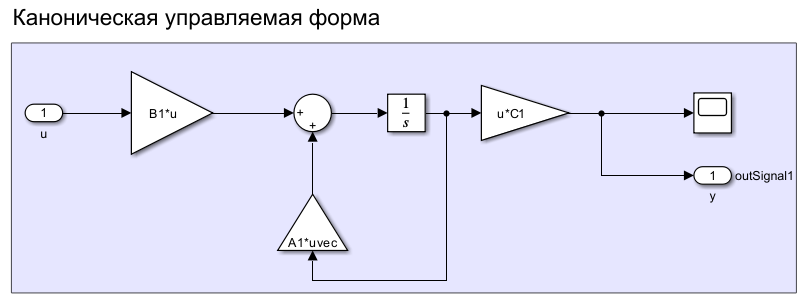
\includegraphics[width=1\textwidth]{scheme_task2_controlled.png}
	\caption{Схема системы - управляемая форма}
\end{figure}
\begin{figure}[ht]
    \centering
    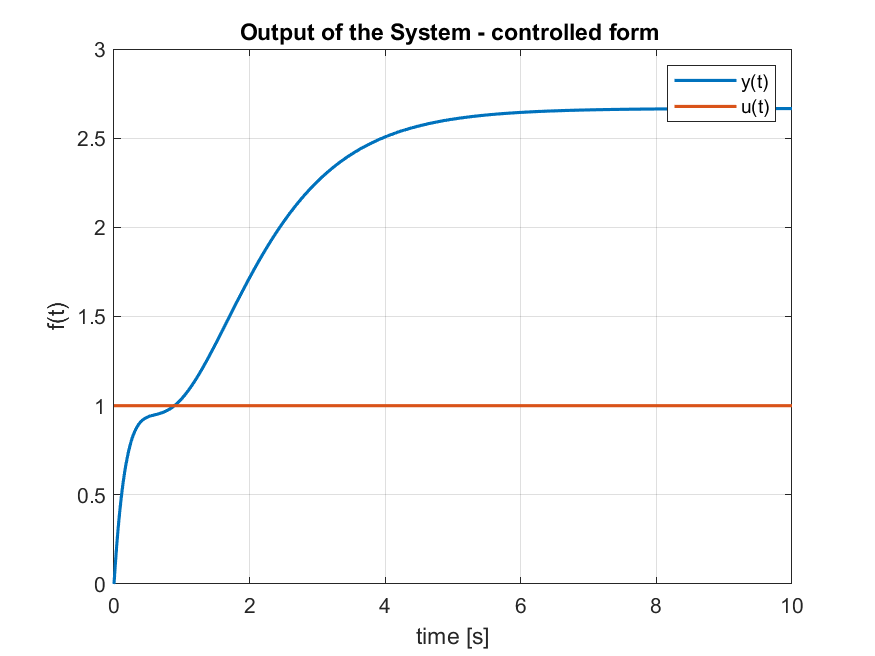
\includegraphics[width=0.5\textwidth]{output_task2_controlled.png}
	\caption{Симуляция - управляемая форма}
\end{figure}

\newpage
\begin{figure}[ht]
    \centering
    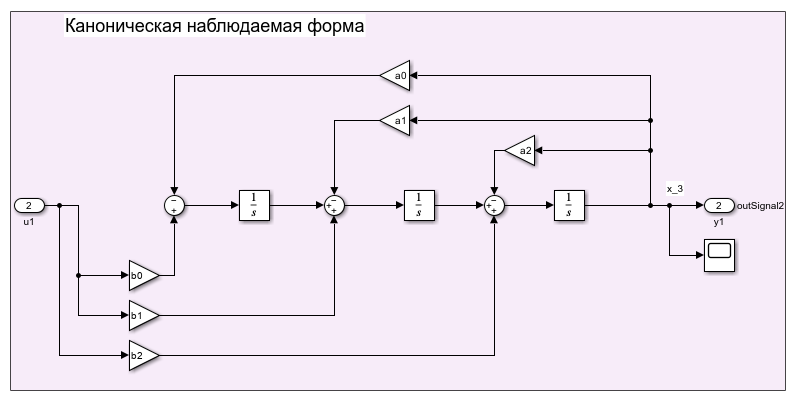
\includegraphics[width=1\textwidth]{scheme_task2_observable.png}
	\caption{Схема системы - наблюдаемая форма}
\end{figure}
\begin{figure}[ht]
    \centering
    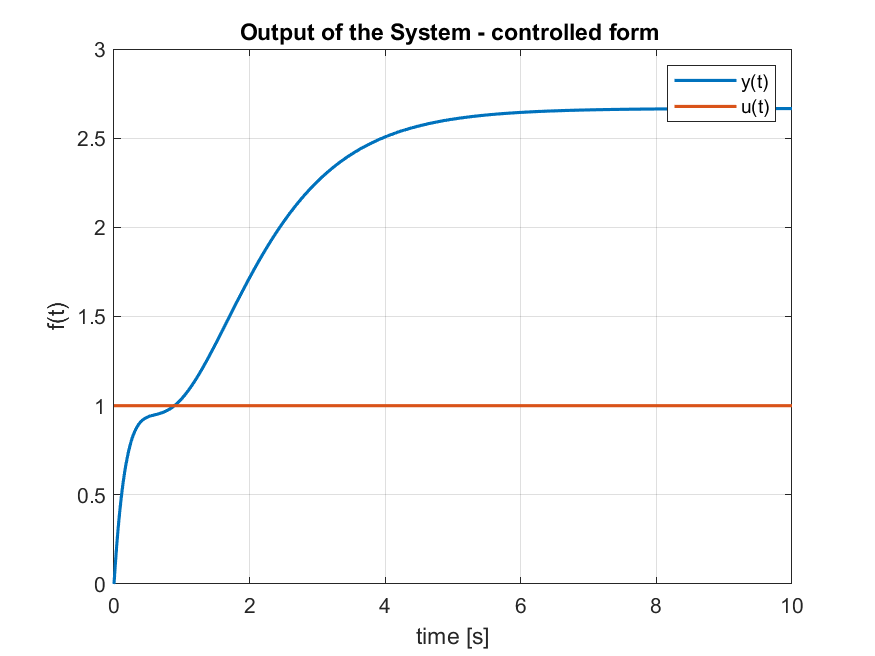
\includegraphics[width=0.5\textwidth]{output_task2_controlled.png}
	\caption{Симуляция - наблюдаемая форма}
\end{figure}

\newpage
\begin{figure}[ht] 
    \centering
    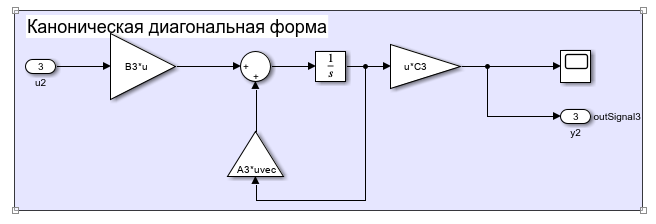
\includegraphics[width=1\textwidth]{scheme_task2_diagonal.png}
	\caption{Схема системы - диагональная форма}
\end{figure}
\begin{figure}[ht]
    \centering
    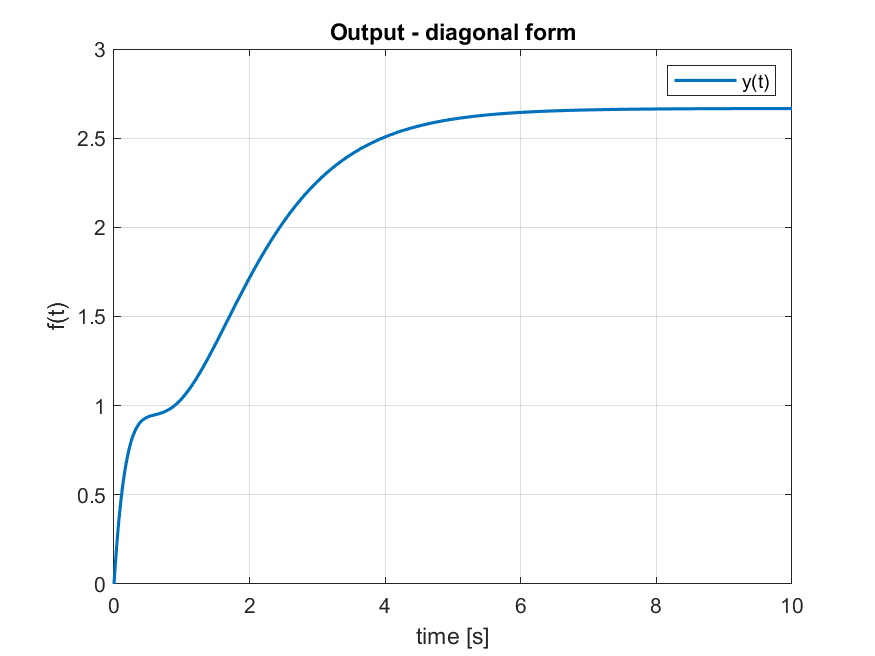
\includegraphics[width=0.5\textwidth]{output_task2_diagonal.png}
	\caption{Симуляция - диагональная форма}
\end{figure}

\section{Выводы}

Невооружённым взглядом видно, что все графики вышли идентичными между собой и по сравнению с формой В-В.

Несложно понять почему это так - ведь мы меняем только вид схемы, меняем точку зрения на систему.

\endinput
\chapter{Многоканальная система в форме вход-выход}
\label{ch:chap3}
\section{Математическая модель системы}


% \begin{itemize}
% 	\item Диагональная форма:
% 	$$
% 	\feqvector{\dot{x_1}, \dot{x_2}, \dot{x_3}} = 
% 	  \begin{bmatrix}
% 		  \lambda_1 & 0 & 0  \\
% 		  0 & \lambda_2 & 0 \\
% 		  0 & 0 & \lambda_3
% 		  \end{bmatrix}
% 	  \feqvector{x_1, x_2, x_3} + \feqvector{\beta_1, \beta_2, \beta_3}u
% 	$$
  
% 	$$
% 	y = \feqvector[&]{\gamma_1, \gamma_2, \gamma_3}\feqvector{x_1, x_2, x_3}
% 	$$
% 	\item С моими коэффициентами:
% 	$$
% 	\feqvector{\dot{x_1}, \dot{x_2}, \dot{x_3}} = 
% 	  \begin{bmatrix}
% 		  -2 & 0 & 0  \\
% 		  0 & -3 & 0 \\
% 		  0 & 0 & -1
% 		  \end{bmatrix}
% 	  \feqvector{x_1, x_2, x_3} + \feqvector{-8, 29, 3}u
% 	$$
  
% 	$$
% 	y = \feqvector[&]{4, 1, 3}\feqvector{x_1, x_2, x_3}
% 	$$
%   \end{itemize}


Рассмотрим следующую систему:
$$
\begin{aligned}
A(p)y(t) = B(p)u(t), \\ где
\end{aligned}
$$

В моём случае у меня будут следующие численные коэффициенты у матриц:

$$
A(p) = \begin{bmatrix}
        p+14 & p+2  \\
        p+7 & p+3 
        \end{bmatrix} , 
B(p) = \begin{bmatrix}
        2 & 8  \\
        9 & 4 
        \end{bmatrix}
$$

Чтобы получить передаточную матрицу (ПМ), немного преобразуем выражение выше:
$$
y(t) = A^{-1}(p)B(p)u(t)
$$

Перемножим и упростим $A^{-1}(p)B(p)$ с помощью матлаба, тогда получим следующее:
$$
W(p) = \begin{bmatrix}
          -\frac{7p+12}{8p+32} & \frac{p+4}{2p+7}  \\
          \frac{7p + 112}{8p + 32} & -\frac{p}{2p+7} 
        \end{bmatrix}
$$

Что и будет являться математической моделью системы.

\section{Структурная схема системы}

Для построения схемы, нам нужно построить четыре передаточных функции - по каждой ячейке передаточной матрицы. 
Также мы знаем, что у нас два входа и выхода - $y_1(t), y_2(t), u_1(t), u_2(t)$:
$$
\feqvector{y_1, y_2} = \begin{bmatrix}
  		  W_{11}(p) & W_{12}(p) \\
  		  W_{21}(p) & W_{22}(p)
  		  \end{bmatrix} 
        \feqvector{u_1, u_2}
$$

Тогда с помошью блоков ПФ получим следующую схему:
\begin{figure}[ht]
  \centering
  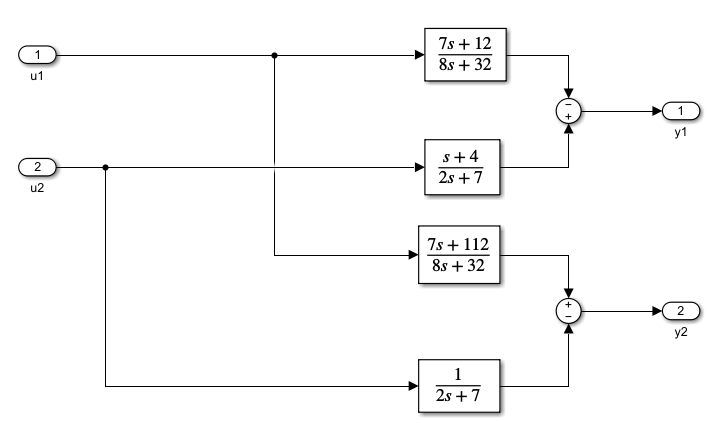
\includegraphics[width=0.6\textwidth]{scheme_task3.png}
\caption{Схема системы - MIMO, EE}
\end{figure}

\section{Графики сигналов u(t) и y(t)}
 
\begin{figure}[ht]
  \centering
  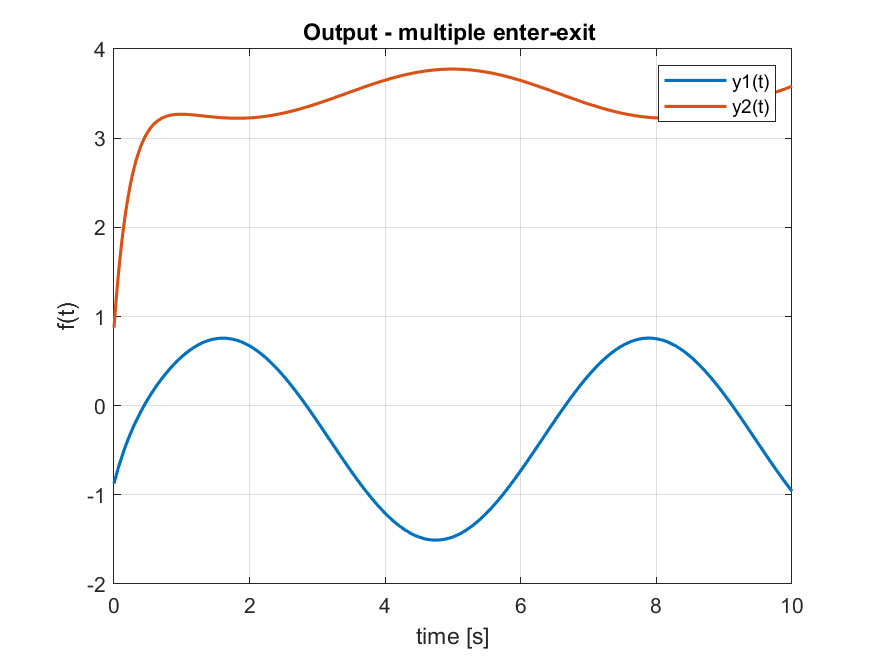
\includegraphics[width=1\textwidth]{output_task3_multiple_EE_1.png}
\caption{Симуляция - $u_1(t) = 1 , u_2(t) = 2sin(t)$}
\end{figure}

\endinput
\chapter{Многоканальная система в форме вход-состояние-выход}
\label{ch:chap4}

\section{Строим структурную схему}

В этом задании мы будем рассматривать систему следующего вида: 
 $$
    \begin{cases}
        x =Ax+Bu,\\
        y = Cx.
    \end{cases}
$$

С учётом моих коэффициентов она превратится в:
$$
\begin{cases}
    \feqvector{\dot{x_1},\dot{x_2}} = \begin{bmatrix}
        0 & -2  \\
        1 & -3 
        \end{bmatrix} \feqvector{x_1,x_2} + \begin{bmatrix}
            2 & 3  \\
            3 & 5 
            \end{bmatrix} \feqvector{u_1,u_2},\\
    y = \begin{bmatrix}
        3 & 5  \\
        4 & 7 
        \end{bmatrix} \feqvector{x_1,x_2}.
\end{cases}
$$

Для удобства построения схемы, перемножим элементы системы и выпишем их:
$$
\begin{aligned}
    \dot{x_1} = -2x_2 + u_1 + 3u_2 \\
    \dot{x_2} = x_1 - 3x_2 + 3u_1 +5u_2 \\
    y_1 = 3x_1 +5x_2 \\
    y_2 = 4x_1 + 7x_2
\end{aligned}
$$
Теперь построить схему стало значительно проще, вот же она:
\begin{figure}[ht]
    \centering
    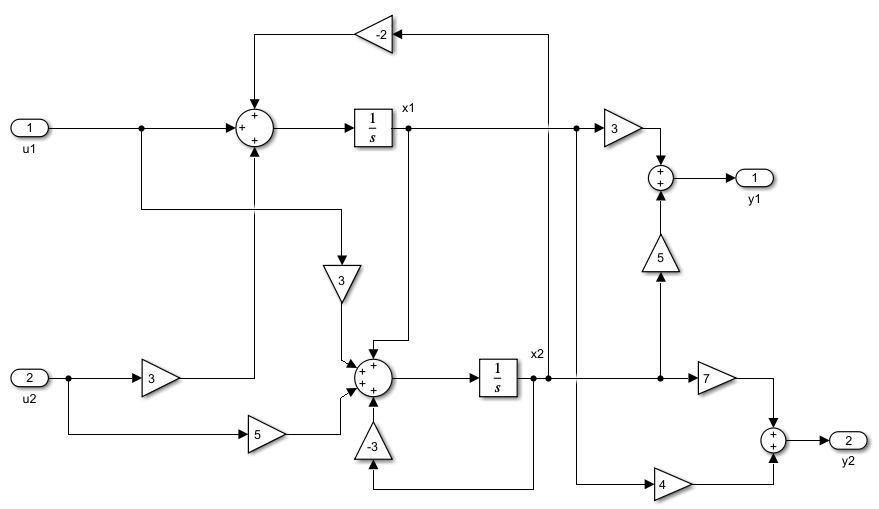
\includegraphics[width=1\textwidth]{scheme_task3_multiple_ECE.png}
  \caption{Схему - MIMO, ECE}
  \end{figure}

\section{Моделируем}

\begin{figure}[ht]
    \centering
    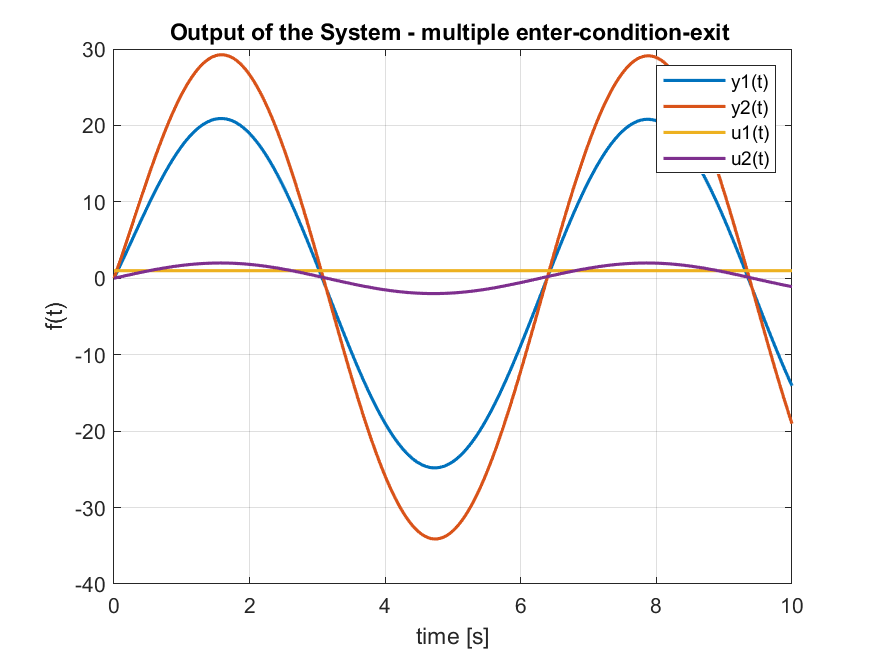
\includegraphics[width=0.6\textwidth]{output_task3_multiple_ECE.png}
  \caption{Симуляция - $u_1(t) = 1 , u_2(t) = 2sin(t)$}
\end{figure}

\endinput 

% \printbibliography[title=Список использованных источников] % Автособираемый список литературы

\end{document}